\documentclass{beamer}
\usefonttheme{professionalfonts}
\RequirePackage{thesis-slides}

\setbeameroption{show notes on second screen=bottom}

\begin{document}
\hspace*{-1.2cm}
\begin{frame}[plain]
\titlepage % Print the title page as the first slide
\end{frame}

\begin{frame}
  \frametitle{Supervised Learning}
  Our idea is to build a theoretical setting that incorporates all the feature real model,
  but at the same time, it's modelized enough to be studied theoretically.
\end{frame}

\begin{frame}
\frametitle{The model: architecture}
Goal: learn a \emph{predictor} \(\hat{f}\) given some samples \((\vec{x},y)\in\Real^{d+1}\).
\vfill
\begin{columns}
  \column{0.4\textwidth}
    \structure{Soft Committee Machine}
    \vspace{1.5pt}

    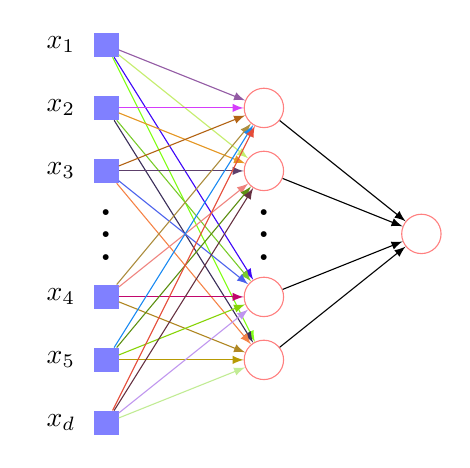
\begin{tikzpicture}[x=1cm, y=.8cm, >=latex]
      \tikzset{
  inputnode/.style={
    rectangle,
    draw,
    minimum size=.3cm
  },
  every neuron/.style={
    circle,
    draw,
    minimum size=.5cm
  },
  neuron missing/.style={
    draw=none, 
    fill=none, %<- added
    scale=2,
    text height=0.333cm,
    execute at begin node=\color{black}$\vdots$
  }
}

\pgfmathparse{rnd}
\xdefinecolor{MyColor}{rgb}{\pgfmathresult, 1.0, 1.0}

\foreach \m [count=\y] in {1,2,3,missing,4,5,6} %<- removed "/\l" here 
  \node [fill=black,inputnode/.try, neuron \m/.try,blue!50] (input-\m) at (0,2.5-\y) {};
% added "fill=green" in the line above

\foreach \m [count=\y] in {1,2,missing,3,4}
  \node [every neuron/.try, neuron \m/.try,red!50] (hidden-\m) at (2,1.5-\y) {};

\foreach \m [count=\y] in {1}
  \node [every neuron/.try, neuron \m/.try,red!50] (output-\m) at (4,-.5-\y) {};

\foreach \l [count=\i] in {1,2,3,4,5,d}
  \path (input-\i) -- ++(-1,0)
   node [midway] {$x_\l$};

% \foreach \l [count=\i] in {1,n}
%   \draw [->] (output-\i) -- ++(1,0)
%    node [above, midway] {$a_\l$};

\foreach \i in {1,...,6}
  \foreach \j in {1,...,4} {
    \edef\R{\pdfuniformdeviate 255}
    \edef\G{\pdfuniformdeviate 255}
    \edef\B{\pdfuniformdeviate 255}
    \xdefinecolor{MyColor}{RGB}{\R,\G,\B}
    \draw [->,MyColor] (input-\i) -- (hidden-\j);
  }


\foreach \i in {1,...,4}
  \foreach \j in {1}
    \draw [->] (hidden-\i) -- (output-\j);

% \foreach \l [count=\x from 0] in {Eingangs-, Ausgangs-}
%   \node [align=center, above] at (\x*4,2) {\l \\ Neuronen};
    \end{tikzpicture}
  \column{0.6\textwidth}
    \[\hat{f}\colon \Real^d\to\Real\]
    \[\hat{f}{(\vec{x})} = \frac{1}{p}\sum_{j=1}^{p} \act{\left(\frac{\vec{w}_j \cdot \vec{x}}{\sqrt{d}}\right)}\]
    \vspace{30pt}

    \begin{center}The network \emph{parameters} are\end{center} 
    \[\vec{w}_j \coloneqq [\W]_j \in \Real^d\]
    \[\W \in \Real^p\times\Real^d\]
\end{columns}
\note[item]{Must define \(d, p, \act\).}
\note[item]{Stress the fact that the \emph{hat} is for the predictor.}
\note[item]{Just one real output, but it's not a problem.}
\note[item]{Fixed weights in the second layer, can be done with more but it's just complicated.
            More parameters, no gain.}
\end{frame}

\begin{frame}
  \frametitle{The model: data samples}
  \(\vec{x}\) samples are \emph{indipendent normal distributions}
  \[
    \vec{x} \sim \gauss{(0,\I_d)}.
  \]
  \pause

  The \(y\) is generated by a \emph{teacher} model with the same architecture
  \[
    f{(\vec{x})} = \frac{1}{k}\sum_{r=1}^{k} \act{\left(\frac{\vec{w}^*_r \cdot \vec{x}}{\sqrt{d}}\right)}
    \quad\text{where}\quad \vec{w}^*_r \coloneqq [\W^*]_r \in \Real^d. 
  \]
  \pause

  We overlap some noise to the \(y\) label
  \[
    y = f{(\vec{x}) + \sqrt{\Delta}\xi}\quad\text{with } \xi \sim \gauss{(0,1)}
  \]
  \note[item]{
    We use Gaussians, but it's not mandatory. It has been done in the past \cite{refinetti2022dynamics}
  }
  \note[item]{
    \emph{Teacher-student setting}: the student knows anything about the architecture of the teacher.
    He observes only pairs. It's just a convenient way of writing a generative model that gives us control on the learning.
  }
  \note[item]{
    teacher has not the hat and the weights matrix has the asterisk
  }
  \note[item]{
    Must say \(\Delta\) is not a parameter of the network, but just a parameter of our theoretical model.
  }
\end{frame}

\begin{frame}
  
\end{frame}








\setbeamertemplate{page number in head/foot}{\phantom{0/0}}
\begin{frame}[noframenumbering, allowframebreaks]
  \frametitle{Bibliography}
  % \textbf{\structure{Bibliography}}
  \printbibliography
  \vspace{3cm}
\end{frame}

\end{document}
